\documentclass[11pt]{article}
\usepackage[margin=2cm]{geometry}
\usepackage[T1]{fontenc}
\usepackage{lmodern}
\usepackage{amsmath}
\usepackage{booktabs}
\usepackage{graphicx}
\usepackage{listings}
\usepackage{algorithm}
\usepackage{algpseudocode}
\usepackage{xcolor}
\usepackage[hidelinks]{hyperref}

\newcommand{\todo}[1]{\textbf{\textcolor{red}{TODO: #1}}}
\lstset{basicstyle=\ttfamily\small, columns=fullflexible}

\begin{document}

% ------------------------------------------------------------------ title
\begin{titlepage}
\centering
\vspace*{3cm}
{\LARGE\bfseries Airport Chaos\par}
\vspace{0.4cm}
{\Large Flight Scheduling \& Crisis Recovery Engine\par}
\vspace{1.2cm}
{\large CP3 Final Project --- CSC310 Algorithms and Data Structures\par}
\vspace{0.3cm}
{\large Instructor: Dr.\ Mohamed Watfa\par}
\vspace{1.5cm}
{\large Lana Fahs \quad ID: 202501399\par}
\vspace{1.5cm}
{\large Submission date: December 1, 2026\par}
\vspace{0.8cm}
{\large GitHub repository:\\[0.2cm]
\href{https://github.com/lanafahs25/ground-stop-scheduler}{\texttt{https://github.com/lanafahs25/ground-stop-scheduler}}\par}
\vfill
{\small Interview commit tag: \texttt{interview-2026-11-28}\par}
\end{titlepage}

% ------------------------------------------------------------------ architecture
\section{Architecture}

The system is a command-line airport scheduler written in Python. It is split
into layers, and each layer has one responsibility:

\begin{enumerate}
  \item \textbf{Data} (\texttt{flight.py}, \texttt{loader.py}): a \texttt{Flight}
  record and a CSV loader that validates every row (timestamp format,
  \texttt{start < end}, priority $\in\{1,2,3\}$, duplicate IDs) and reports bad
  rows with their line number instead of stopping. Each flight also keeps its
  original times (\texttt{orig\_start}, \texttt{orig\_end}) so that later
  analysis can refer to the original schedule after delays.
  \item \textbf{Storage}: a hash registry (\texttt{registry.py}) holding
  \emph{every} flight by ID, and one binary search tree per runway
  (\texttt{bst.py}) holding only the \emph{active} (non-cancelled) flights,
  ordered by time.
  \item \textbf{Engine} (\texttt{engine.py}): the only component allowed to
  modify the registry and the trees. Every operation (load, add, cancel,
  reschedule) goes through it, which is how the two structures are kept
  synchronised.
  \item \textbf{Interface} (\texttt{cli.py}): an interactive numbered menu, a
  batch runner for command files, and a single-command mode, all built on one
  command parser and exposed through a Typer entry point
  (\texttt{python cli.py menu | batch FILE | run "COMMAND"}). A \texttt{TRACE}
  switch prints hash probes, BST search paths and neighbours, and sorting
  passes. The CLI only calls engine and algorithm functions; it contains no
  algorithm logic. An optional Tkinter GUI (\texttt{gui/app.py}) shows the
  runway timelines, scenario results, disruption chart and route heatmap on
  top of the same engine.
\end{enumerate}

Runways are not hard-coded: the engine creates one tree per runway name found in
the data, so files with other runways work unchanged.

% ------------------------------------------------------------------ mapping
\section{Module-to-algorithm mapping}

\begin{center}
\begin{tabular}{@{}lll@{}}
\toprule
Requirement & File & Algorithm / structure \\
\midrule
A. Flight registry & \texttt{registry.py} & Universal hashing, linear probing, tombstones, resizing \\
B. Runway scheduler & \texttt{bst.py} & Unbalanced BST, floor/ceiling, range search \\
Synchronisation & \texttt{engine.py} & Engine layer + consistency check \\
C. Crisis scenarios & \texttt{engine.py} & Greedy recovery rule, conflict search, range search \\
D. Sorting & \texttt{sorting.py} & Counting sort, LSD radix sort \\
E. Disruption analysis & \texttt{analysis.py} & Divide-and-conquer maximum subarray \\
F. Route matrix & \texttt{matrix.py} & Classical and Strassen multiplication \\
G. Rule IDs & \texttt{perfect\_hash.py} & FKS two-level perfect hashing \\
\bottomrule
\end{tabular}
\end{center}

% ------------------------------------------------------------------ A
\section{A. Flight registry: universal hashing with open addressing}

\subsection{Encoding IDs as integers}
Flight IDs are alphanumeric strings, so each ID is first turned into an integer
with a polynomial encoding in base 131:
\[
k = \Bigl(\sum_{i} \mathrm{ord}(c_i)\cdot 131^{\,n-1-i}\Bigr) \bmod p .
\]
Base 131 is larger than the largest character code used in IDs
(\texttt{z} = 122), so the encoding behaves like a number written in base 131
and different IDs give different integers. Since $131^8 < p$, the encoding is
exactly injective for IDs of up to 8 characters; all official IDs have 7.
A smaller base such as 31 would not be injective:
\texttt{"Ab"} and \texttt{"BC"} both encode to 2113.
Lookups still compare the full original ID strings, so even an encoding
collision on longer IDs could never return the wrong flight.

\subsection{Universal hash function}
\[
h(k) = \bigl((a\cdot k + b) \bmod p\bigr) \bmod m,
\qquad p = 2^{61}-1,\; a \in [1,p-1],\; b\in[0,p-1].
\]
$p$ is a Mersenne prime, which satisfies the two conditions of universal hashing
(CLRS \S11.3.3): it is prime, and it is larger than every encoded key.
$a$ and $b$ are drawn once from \texttt{random.Random(42)}, so the function is
random with respect to the input but the program is deterministic across runs.
The table starts with $m = 16$ slots.

\subsection{Linear probing, tombstones and resizing}
Collisions are resolved with linear probing: if slot $i$ is taken, try
$(i+1) \bmod m$. A slot is either empty, a flight, or a \emph{tombstone}.

\begin{itemize}
  \item \textbf{Lookup} walks from $h(k)$ and stops at the matching ID or at an
  empty slot. Tombstones are stepped over, because the target may lie further
  along the probe chain.
  \item \textbf{Delete} replaces the flight with a tombstone instead of emptying
  the slot. Emptying it would break the probe chain: a later flight that was
  pushed past this slot by a collision would become unreachable.
  \item \textbf{Insert} remembers the first tombstone it passes but keeps
  scanning until an empty slot, to make sure the ID is not already stored
  further along. It then places the flight in that first tombstone if there
  was one, otherwise in the empty slot. Duplicate IDs are rejected.
  \item \textbf{Resize}: before each insert, if
  $(\text{size}+\text{tombstones}+1)/m > 0.6$, the table doubles and every
  flight is reinserted. Tombstones are counted because they occupy slots and
  lengthen probe chains; resizing also discards them. Flights must be
  reinserted rather than copied to the same index, because their slot depends
  on $m$.
  \item Every loop is bounded by $m$ probes, so a full table raises an error
  instead of looping forever (resizing prevents this in practice).
\end{itemize}

\begin{algorithm}[ht]
\caption{Registry insert (matches \texttt{HashRegistry.insert})}
\begin{algorithmic}[1]
\Procedure{Insert}{$f$}
  \If{$(\mathit{size}+\mathit{tombstones}+1)/m > 0.6$} \Call{Resize}{} \EndIf
  \State $i \gets h(f.\mathit{id})$; \quad $\mathit{firstTomb} \gets \textsc{nil}$
  \For{$j \gets 1$ \textbf{to} $m$}
    \If{$T[i] = \textsc{nil}$}
      \If{$\mathit{firstTomb} \neq \textsc{nil}$}
        \State $T[\mathit{firstTomb}] \gets f$; \quad $\mathit{tombstones} \gets \mathit{tombstones}-1$
      \Else
        \State $T[i] \gets f$
      \EndIf
      \State $\mathit{size} \gets \mathit{size}+1$; \Return \textsc{true}
    \ElsIf{$T[i] = \textsc{tomb}$}
      \If{$\mathit{firstTomb} = \textsc{nil}$} $\mathit{firstTomb} \gets i$ \EndIf
    \ElsIf{$T[i].\mathit{id} = f.\mathit{id}$}
      \State \Return \textsc{false} \Comment{duplicate}
    \EndIf
    \State $\mathit{collisions} \gets \mathit{collisions}+1$; \quad $i \gets (i+1) \bmod m$
  \EndFor
  \If{$\mathit{firstTomb} \neq \textsc{nil}$}
    \State $T[\mathit{firstTomb}] \gets f$; update counters; \Return \textsc{true}
  \EndIf
  \State \textbf{error} ``table full''
\EndProcedure
\end{algorithmic}
\end{algorithm}

\begin{algorithm}[ht]
\caption{Registry lookup and delete (match \texttt{lookup}, \texttt{delete})}
\begin{algorithmic}[1]
\Procedure{Lookup}{$\mathit{id}$}
  \State $i \gets h(\mathit{id})$; \quad $\mathit{probes} \gets 0$
  \For{$j \gets 1$ \textbf{to} $m$}
    \State $\mathit{probes} \gets \mathit{probes}+1$
    \If{$T[i] = \textsc{nil}$} \Return $(\textsc{nil}, \mathit{probes})$
    \ElsIf{$T[i] \neq \textsc{tomb}$ \textbf{and} $T[i].\mathit{id} = \mathit{id}$} \Return $(T[i], \mathit{probes})$
    \EndIf
    \State $i \gets (i+1) \bmod m$
  \EndFor
  \State \Return $(\textsc{nil}, \mathit{probes})$
\EndProcedure
\Statex
\Procedure{Delete}{$\mathit{id}$}
  \State walk as in \textsc{Lookup}; on a match: $T[i] \gets \textsc{tomb}$,
  $\mathit{size} \gets \mathit{size}-1$, $\mathit{tombstones} \gets \mathit{tombstones}+1$
\EndProcedure
\end{algorithmic}
\end{algorithm}

\subsection{Measured behaviour on the official file}
After loading all 1{,}000 flights the table has grown from 16 to 2{,}048 slots
(7 resizes) and has load factor $\alpha = 0.488$. Looking up all 1{,}000 IDs
took on average \textbf{1.67 probes} per lookup.
For comparison, the classical estimate for a successful search with linear
probing is $\tfrac12\bigl(1 + \tfrac{1}{1-\alpha}\bigr) \approx 1.48$ at this
load factor, so the measurement is close to theory.
The collision counter reports 5{,}583; this includes the collisions that happen
while flights are reinserted during the 7 resizes, not only those of the final
table.

% ------------------------------------------------------------------ B
\section{B. Runway scheduler: one BST per runway}

\subsection{Keys and invariant}
Each runway has its own unbalanced BST. A node stores the key
$(\mathit{start}, \mathit{flight\_id})$, the end time and a reference to the
flight. Using the pair as the key makes every key unique, and Python compares
tuples lexicographically (start first, then ID). Each node also stores a parent
pointer, which successor, predecessor and delete use to walk upwards.

\textbf{Invariant:} the flights in a runway tree never overlap. Intervals are
half-open, $[\mathit{start}, \mathit{end})$, so a flight ending at 09:20 does
not conflict with one starting at 09:20. Different runways have separate trees,
so they can never conflict.

All operations are written iteratively (loops and an explicit stack for the
inorder walk), so a degenerate tree cannot exceed Python's recursion limit.

\subsection{Operations}
\begin{itemize}
  \item \textbf{Insert, search, minimum, maximum, successor, predecessor}:
  standard CLRS algorithms (\S12.2--12.3), $O(h)$.
  \item \textbf{Inorder}: iterative with an explicit stack; returns the runway
  schedule in time order, $O(n)$.
  \item \textbf{Delete}: the three CLRS cases using a \textsc{Transplant} helper;
  a node with two children is replaced by its successor. Root deletion is
  handled by \textsc{Transplant} when the node has no parent.
  \item \textbf{Range search} $[t_1, t_2)$: an inorder walk that skips left
  subtrees whose root starts before $t_1$ and stops at the first node starting
  at or after $t_2$; $O(h + k)$ for $k$ results.
  \item \textbf{Floor / ceiling}$(t)$: the node with the latest start $\le t$ /
  the earliest start $\ge t$, i.e.\ predecessor and successor of a time that is
  not itself in the tree; $O(h)$.
  \item \textbf{Height}: computed level by level; $O(n)$.
\end{itemize}

\subsection{Conflict check}
To test a proposed interval $[s, e)$ against a conflict-free runway, only two
kinds of flight can overlap it:
\begin{enumerate}
  \item a flight that started \emph{before} $s$ and is still running. Because the
  schedule has no overlaps, only the latest such flight can still be running,
  which is $\textsc{Floor}(s)$;
  \item flights that start \emph{inside} $[s, e)$, found by range search.
\end{enumerate}

\begin{algorithm}[ht]
\caption{Conflict check (matches \texttt{RunwayBST.conflicts})}
\begin{algorithmic}[1]
\Procedure{Conflicts}{$s, e$}
  \State $R \gets [\,]$; \quad $f \gets \Call{Floor}{s}$
  \If{$f \neq \textsc{nil}$ \textbf{and} $f.\mathit{start} < s$ \textbf{and} $f.\mathit{end} > s$}
    \State append $f$ to $R$
  \EndIf
  \State append \Call{RangeSearch}{$s, e$} to $R$
  \State \Return $R$ \Comment{empty means the slot is free}
\EndProcedure
\end{algorithmic}
\end{algorithm}

The strict test $f.\mathit{start} < s$ prevents a flight starting exactly at $s$
from being listed twice, since range search already includes it. The test
$f.\mathit{end} > s$ implements the half-open boundary. The total cost is
$O(h + k)$.

\subsection{Measured tree heights}
For 200 flights a perfectly balanced tree would have height
$\lceil \log_2 201 \rceil = 8$, and a degenerate chain would have height 200.
Loading the official file (whose rows are in random time order) gives:

\begin{center}
\begin{tabular}{@{}lccccc@{}}
\toprule
Runway & R1 & R2 & R3 & R4 & R5 \\
\midrule
Flights & 200 & 200 & 200 & 200 & 200 \\
Height  & 16 & 15 & 14 & 16 & 14 \\
\bottomrule
\end{tabular}
\end{center}

Reinserting the R1 flights in sorted time order produces a tree of height
\textbf{200}, the $O(n)$ worst case of an unbalanced BST.
Timings for sorted versus shuffled insertion (up to $146\times$ slower searches) are in Section~\ref{sec:bench}.

% ------------------------------------------------------------------ engine
\section{Engine and consistency}

The engine owns one registry and one tree per runway, and every change goes
through it.

\begin{itemize}
  \item \textbf{Load} starts from fresh structures every time (so each scenario
  can be run from a clean state), and checks each flight against its runway
  tree before inserting it. A flight that would overlap an earlier one is
  skipped and reported, so the no-overlap invariant holds even for an
  unexpected input file.
  \item \textbf{Add} checks for a duplicate ID and for runway conflicts first,
  and only modifies the structures when every check passes, returning the
  conflicting flights otherwise.
  \item \textbf{Cancel} removes the flight from its runway tree, so it no longer
  blocks the runway, but keeps it in the registry with status
  \texttt{CANCELLED}.
  \item \textbf{Reschedule} keeps the flight's duration and runway. It first
  removes the flight from its tree (otherwise it would conflict with its own old
  slot), then checks the new interval. On a conflict the flight is reinserted
  with its unchanged times (rollback); otherwise its times are updated and it is
  reinserted. The registry needs no change, because it is keyed by ID and holds
  a reference to the same flight object.
  \item \textbf{Consistency check} verifies that every tree node is active, on
  the right runway, has a key matching the flight's current times, and is the
  same object the registry returns, and that the number of tree nodes equals
  the number of active flights in the registry. It returns a list of problems
  (empty means consistent) and is used by the tests after every kind of update.
\end{itemize}

% ------------------------------------------------------------------ remaining
\section{C. Crisis scenarios}

The three scenarios are engine methods
(\texttt{runway\_closure}, \texttt{emergency\_insert},
\texttt{mass\_cancel}) built from the BST operations of Section~4. They take
the runway and times as parameters, so nothing is specific to the official
file. Each official result below was produced from a fresh load.

\subsection{Recovery rule (runway closure)}
Affected flights are the flights on the closed runway whose occupancy
intersects $[c_s, c_e)$, which is exactly \textsc{Conflicts}$(c_s, c_e)$. They
are processed as follows:

\begin{enumerate}
  \item \textbf{Remove all affected flights from the tree first.} Otherwise
  their old slots inside the closed window would block the new slots they are
  competing for, causing unnecessary delays and breaking the priority order.
  The only flights left in the tree are unaffected ones, which are never moved.
  \item \textbf{Order} them by (priority, original start, flight\_id) with an
  insertion sort on that tuple; the list is small, so $O(k^2)$ is negligible.
  \item For each flight, try start times $c_e, c_e+5, c_e+10, \dots$ minutes,
  keeping its duration. The first conflict-free slot is taken (status
  \texttt{DELAYED}) and the flight is reinserted, so later flights see it. If
  the delay from its original start would exceed 120 minutes, the flight is
  \texttt{CANCELLED} instead; it stays out of the tree but remains in the
  registry.
\end{enumerate}

\begin{algorithm}[ht]
\caption{Runway closure (matches \texttt{Engine.runway\_closure})}
\begin{algorithmic}[1]
\Procedure{RunwayClosure}{$r, c_s, c_e$}
  \State $T \gets$ tree of runway $r$; \quad $A \gets$ \textsc{Conflicts}$(c_s, c_e)$ on $T$
  \For{each $f \in A$} \State delete $f$'s node from $T$ \EndFor
  \State insertion-sort $A$ by $(f.\mathit{priority}, f.\mathit{origStart}, f.\mathit{id})$
  \For{each $f \in A$}
    \State $d \gets f.\mathit{end} - f.\mathit{start}$; \quad $t \gets c_e$
    \While{$t - f.\mathit{origStart} \le 120$ min}
      \If{\textsc{Conflicts}$(t, t+d)$ on $T$ is empty}
        \State $f.\mathit{start} \gets t$; $f.\mathit{end} \gets t+d$; status \texttt{DELAYED};
        insert $f$ into $T$; \textbf{break}
      \EndIf
      \State $t \gets t + 5$ min
    \EndWhile
    \If{$f$ was not placed} status \texttt{CANCELLED} \EndIf
  \EndFor
  \State \Return rows (ID, old time, new time, status) and totals
\EndProcedure
\end{algorithmic}
\end{algorithm}

\subsection{Official results}

\paragraph{Scenario A --- RUNWAY\_CLOSURE R1 09:00--11:00.}
18 flights are affected. This includes F910078 (08:59--09:04), which starts
before the closure but is still on the runway at 09:00 and is found by the
\textsc{Floor} part of the conflict check.

\begin{center}
\begin{tabular}{@{}lc@{}}
\toprule
Affected & 18 \\
Delayed & 1 (BA10079, 09:06 $\to$ 11:00, 114 min) \\
Cancelled & 17 \\
Total delay & 114 min \\
Consistency check after scenario & passed \\
\bottomrule
\end{tabular}
\end{center}

Removing all 18 affected flights frees 08:59--11:03, so the slot 11:00--11:05
becomes available and goes to the highest-priority, earliest flight. Every
other affected flight is cancelled because R1 is occupied for 1{,}000 of the
day's 1{,}440 minutes, with gaps of about 2 minutes between flights after 11:05:
no 5-minute slot exists within any flight's 120-minute limit. This was
confirmed independently from the raw CSV.

The full per-flight table is in Appendix~\ref{app:scenario}.

\paragraph{Scenario B --- EMERGENCY\_INSERT EM90001, R1, 09:00--09:05, priority 1.}
The requested slot conflicts with \textbf{F910078} (08:59--09:04). No existing
flight is moved: the method searches forward from the requested start in
5-minute steps and offers the earliest conflict-free slot, \textbf{23:20}.
Without confirmation nothing is inserted; with confirmation (\texttt{ACCEPT})
EM90001 is inserted at 23:20--23:25 and the consistency check passes. The
handout gives no limit for this search, so the implementation stops after
24 hours and reports that no slot exists. The late offer has the same cause
as above: the first 5-minute gap on R1 after 09:00 opens at 23:18, and the
first start on the 5-minute grid is 23:20.

\paragraph{Scenario C --- MASS\_CANCEL 14:00--15:00.}
Range search $[14{:}00, 15{:}00)$ on every runway finds \textbf{45} flights,
9 per runway, matching a direct count from the CSV. All are removed from the
trees and kept in the registry as \texttt{CANCELLED}; active flights drop from
1{,}000 to 955 and the consistency check passes. Range search (start time)
is used here rather than the conflict check (overlap), because the rule
cancels flights whose \emph{start} lies in the window: a flight starting at
13:58 is not cancelled.


\section{D. Counting sort, radix sort and the lower bound}

\subsection{Counting sort on priority}
Priorities take only $k = 3$ values, so the flights are sorted without
comparing them: count how many flights have each priority, turn the counts
into running totals (so \texttt{count[p]} is the position just after the last
slot of group $p$), then place each flight directly into its group. The input
is scanned \emph{from the back} and each group is filled from its last slot,
so flights with equal priority keep their input order: the sort is
\textbf{stable}. Cost $\Theta(n + k)$.

\subsection{LSD radix sort on flight IDs}
IDs are sorted character by character, from the \emph{last} position to the
first, with a stable counting sort at each position (CLRS \S8.3). Each
character is mapped to \texttt{ord(c)+1} ($1..128$, $k = 128$); a position past
the end of a shorter ID maps to $0$, so a prefix sorts first (\texttt{"AB"}
$<$ \texttt{"ABC"}) and the result is exact lexicographic order of the
original strings, with no numeric encoding and therefore no collisions. With
$d$ the longest ID length the cost is $\Theta(d(n + k))$; for the official
file $d = 7$.

\subsection{Stability example}
\texttt{SORT\_DEMO} sorts all 1{,}000 flights by ID with radix sort and then by
priority with counting sort. Because counting sort is stable, flights inside
each priority group remain in ID order; the program checks this over the whole
list and reports \texttt{True}. The automated tests also check stability
against the original input positions.

\subsection{Lower bound for comparison sorting}
Any comparison sort can be modelled as a binary decision tree whose internal
nodes are comparisons $a_i \le a_j$ and whose leaves are output orders. A
correct sort must be able to produce all $n!$ orders, so the tree has at least
$n!$ leaves and its height is at least $\log_2(n!) = \Omega(n \log n)$
(Stirling). The height is the worst-case number of comparisons, so every
comparison sort needs $\Omega(n \log n)$ comparisons in the worst case.
Counting and radix sort are outside this model: they never compare two keys,
they use key values as array indices. Their cost depends on the key range $k$
and the number of digits $d$, giving $\Theta(n + k)$ and $\Theta(d(n+k))$,
which is linear when $k$ and $d$ are small, as here.

\section{E. Divide-and-conquer disruption analysis}

\paragraph{Load array.}
The simulation date is taken from the data (the date of the earliest original
start), and divided into 288 five-minute buckets. Bucket $i$ counts the flights
whose \emph{original} start (\texttt{orig\_start}) falls in
$[\,5i, 5i+5)$ minutes after midnight and whose current status is
\texttt{DELAYED} or \texttt{CANCELLED}. Using the original start means a delayed
flight is counted where the disruption happened, not where it moved to.

\paragraph{Algorithm.}
CLRS \textsc{Find-Maximum-Subarray}: split at the middle; the best range lies
entirely in the left half, entirely in the right half (both solved
recursively), or crosses the middle. The crossing case is the best sum ending
at \textit{mid} plus the best sum starting at $\textit{mid}+1$, found by two
linear scans outward. The result is the largest of the three. The recurrence is
\[
T(n) = 2\,T(n/2) + \Theta(n) \;\Rightarrow\; T(n) = \Theta(n \log n)
\]
by case 2 of the Master theorem. Recursion depth is only $\lceil\log_2 288\rceil = 9$.
An $O(n^2)$ reference tries every start and end with a running total.

\paragraph{Ties and the all-zero array.}
Several ranges can share the maximum sum (for example by including zero
buckets at an edge), so both results are normalised the same way: zero buckets
are trimmed from both ends. If the maximum sum is $0$ (no disrupted flight),
the program reports that there is nothing to analyse.

\paragraph{Results.}
After a fresh load the array is all zero and \texttt{ANALYZE} reports no
disruption. After scenario A, the maximum range is buckets
\textbf{107--131} (08:55--11:00) with \textbf{18} disrupted flights, and the
$O(n^2)$ reference agrees. Because loads are counts and never negative, the
maximum range always runs from the first to the last disrupted bucket; the
algorithm is still the general one, and it is verified on the CLRS example
(which has negative values, answer indices 7--10, sum 43) and on 200 random
arrays against the reference.

\section{F. Classical and Strassen multiplication}

\paragraph{Route matrix.}
The 14 airports of the official file, in lexicographic order
(ATL, BOS, CLT, DEN, DFW, IAD, JFK, LAS, LAX, MIA, ORD, PHX, SEA, SFO), index
the rows and columns of $A$, where $A_{ij}$ is the number of flights from $i$
to $j$ in the original schedule (all 1{,}000 flights). Then
$(A^2)_{ij} = \sum_k A_{ik}A_{kj}$ counts two-leg combinations $i \to k \to j$.
It ignores times, so it is a route-count proxy, not a count of feasible
connections. The largest entry is \textbf{ORD $\to$ LAS with 600
combinations}, which was confirmed independently from the raw CSV.

\paragraph{Classical.} The triple loop, $\Theta(N^3)$.

\paragraph{Strassen.}
Each matrix is split into four quarters and the product is assembled from
seven half-size products instead of eight (CLRS \S4.2), at the cost of
$\Theta(N^2)$ extra additions:
\[
T(N) = 7\,T(N/2) + \Theta(N^2) \;\Rightarrow\; T(N) = \Theta(N^{\log_2 7}) \approx \Theta(N^{2.81}).
\]
Matrices are zero-padded up to the next power of two (14 $\to$ 16), multiplied,
and cropped back; the padding only produces zeros outside the original
block. Below a documented \textbf{cutoff of 32} the recursion switches to the
classical algorithm. Correctness is tested with \texttt{cutoff=1} (full
recursion) on random matrices of sizes 1, 2, 3, 5, 7, 8, 13, 16 and 33 and on
the route matrix; all match the classical result exactly.

\paragraph{Why Strassen can lose for small $N$.}
Each level allocates and adds many temporary matrices, and Python's
per-operation overhead is large, so the saved multiplication only pays off
once blocks are big. With the cutoff, the 16$\times$16 route matrix never
recurses at all. The measured crossover is discussed in
Section~\ref{sec:bench}.

\section{G. Static perfect hashing}

The 20 fixed rule IDs
(101, 107, \ldots, 283) are stored with two-level FKS hashing (CLRS \S11.5).
Both levels use the universal family $h(k) = ((ak+b) \bmod p) \bmod m$ with
$p = 293$, a prime larger than every key, and $a, b$ drawn from a seeded
generator.

\begin{itemize}
  \item \textbf{Level 1}: hash the $n = 20$ keys into $m = 20$ buckets.
  Parameters are re-chosen until $\sum s_j^2 \le 4n$, where $s_j$ is the bucket
  size; this keeps total storage $O(n)$ and succeeds with probability at least
  $1/2$ per try.
  \item \textbf{Level 2}: a bucket with $s$ keys gets its own table of size
  $s^2$ and its own $(a,b)$, re-chosen until there are no collisions
  (probability at least $1/2$ per try).
  \item \textbf{Lookup}: two hash computations and one key comparison, so
  $O(1)$ in the \emph{worst} case. Comparing the stored key rejects absent IDs
  that hash to an occupied slot.
\end{itemize}

\paragraph{Results.}
Bucket sizes: three buckets of 2, two of 3, eight of 1 and seven empty.
Storage is \textbf{58 slots} (20 for level 1 plus $\sum s_j^2 = 38$), within
the $20 + 4n = 100$ bound. Level 1 succeeded on the first try; level 2 needed
2 re-draws in total. All 20 IDs are found; 100, 102, 284 and 999 are correctly
reported absent (\texttt{RULES} command).

\section{Testing}

\texttt{python -m unittest -v} runs 23 automated tests (\texttt{tests/test\_all.py}),
all passing:

Table~\ref{tab:tests} in Appendix~\ref{app:tests} lists them; they cover:
loader validation, registry collisions/tombstones/resize, BST root deletion
and neighbours, the exact boundary case, cross-runway independence, conflict
rejection, all three scenarios from a fresh load, sorting stability, maximum
subarray against the $O(n^2)$ reference, Strassen on odd sizes, consistency
after updates, and perfect hashing.

The scenario tests are regression tests: they fix the official outputs
(18/1/17 with 114 minutes; F910078 and the 23:20 slot; 45 cancellations) so any
change that alters them fails. The program itself never hard-codes these
results.

\section{Benchmarks}\label{sec:bench}

\texttt{python benchmarks/run\_benchmarks.py} runs four experiments on
synthetic data with fixed seeds and writes \texttt{benchmarks/results/*.csv}
and \texttt{benchmarks/plots/*.png}. \textbf{Environment:} CPython 3.13.5 on
macOS 27 (Apple Silicon, arm64). Each timing is the median of 5 repeats
(1 repeat for the $256\times256$ matrices). The official CSV is used only for
correctness; scale experiments use generated flights.

\begin{figure}[ht]\centering
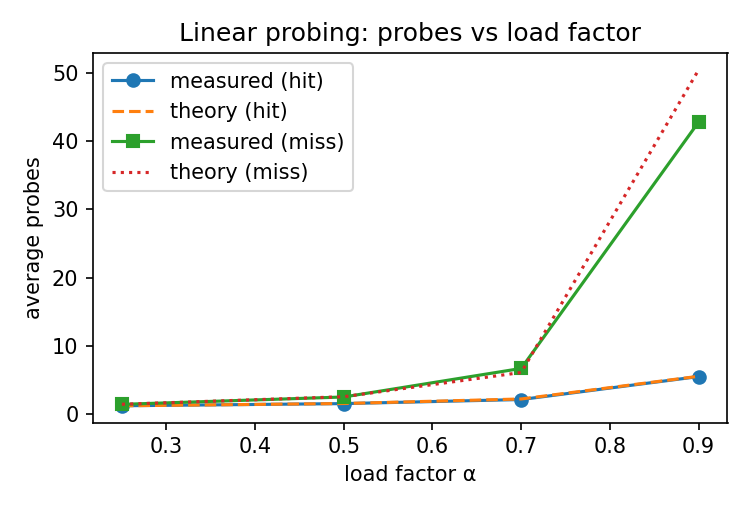
\includegraphics[width=0.49\textwidth]{../benchmarks/plots/hash_load_factor.png}
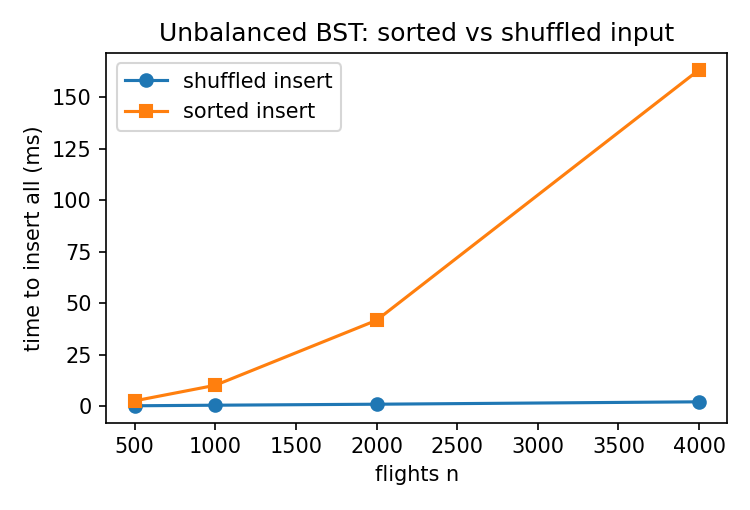
\includegraphics[width=0.49\textwidth]{../benchmarks/plots/bst_sorted_vs_shuffled.png}\\[4pt]
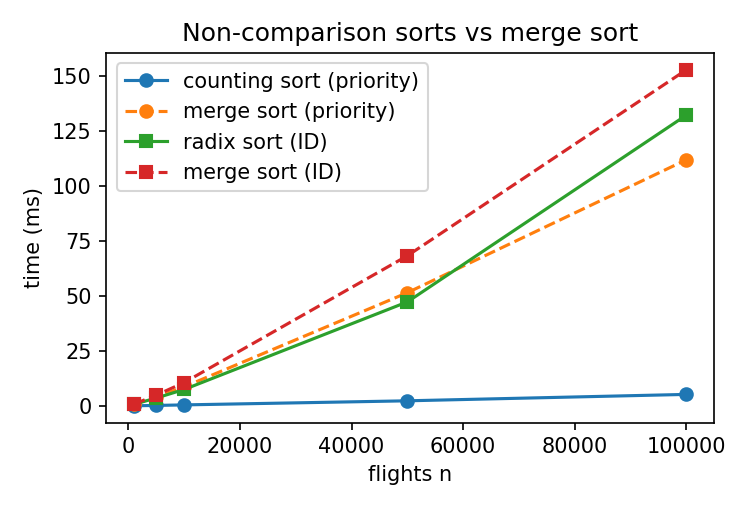
\includegraphics[width=0.49\textwidth]{../benchmarks/plots/sorting.png}
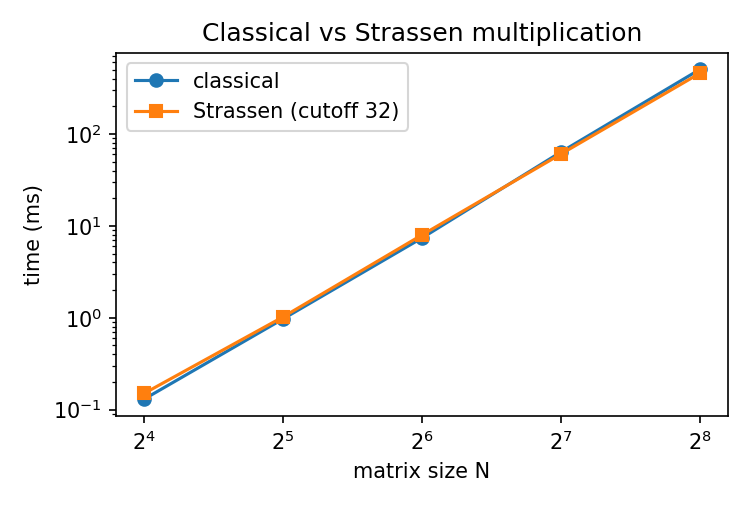
\includegraphics[width=0.49\textwidth]{../benchmarks/plots/matrix.png}
\caption{Benchmark results (data in \texttt{benchmarks/results/}).}
\end{figure}

\subsection{Hash lookups vs load factor}
Table size fixed at $m = 8192$ (resizing disabled for this experiment only); numbers in Table~\ref{tab:bhash}.
Measurements follow the linear-probing estimates
$\frac12(1+\frac{1}{1-\alpha})$ (hit) and $\frac12(1+\frac{1}{(1-\alpha)^2})$
(miss) closely. Unsuccessful searches grow fastest: about 43 probes at
$\alpha = 0.9$ against 2.5 at $\alpha = 0.5$. This is the reason the registry
resizes at $\alpha = 0.6$. Time per lookup stays around 1--2\,$\mu$s.

\subsection{BST: sorted vs shuffled insertion}
(Table~\ref{tab:bbst}.)
Shuffled input gives heights close to $2\log_2 n$ and near-linear growth of the
total time. Sorted input produces a chain of height $n$: every operation is
$O(n)$, so building and searching all keys become $O(n^2)$, and doubling $n$
multiplies the time by about 4. At $n = 4000$, searching every key is about
$146\times$ slower than on the shuffled tree.

\subsection{Counting and radix sort vs merge sort}
(Table~\ref{tab:bsort}.)
Times in ms. Counting sort ($k = 3$) is about $20\times$ faster than merge sort
and grows linearly. Radix sort is faster than merge sort on the same IDs at
every size, but only by 10--30\%: it makes $d = 7$ passes, each scanning a
count array of size $k = 128$, so its constant factor is large, while
$\log_2 n$ at these sizes is only 10--17.

\subsection{Classical vs Strassen}
(Table~\ref{tab:bmat}.)
Times in ms. Both grow by roughly $8\times$ per doubling at these sizes.
Strassen with cutoff 32 only breaks even at $N = 128$ and is about 4\% faster
at $N = 256$. Recursing all the way down (cutoff 1) is 15--17$\times$ slower,
because every level allocates and adds temporary matrices in Python, which
costs more than the multiplication it saves. The asymptotic advantage
($N^{2.81}$ vs $N^3$) needs much larger matrices, or a lower-overhead
language, to show.

\section{Complexity summary}

\begin{center}
\begin{tabular}{@{}lll@{}}
\toprule
Operation & Average & Worst case \\
\midrule
Registry insert / lookup / delete & $O(1)$ expected ($\alpha \le 0.6$) & $O(m)$ \\
Registry resize & $O(m)$, amortised $O(1)$ per insert & $O(m)$ \\
BST insert / search / delete & $O(h)$, $h = O(\log n)$ for random order & $O(n)$ \\
BST successor / predecessor / floor / ceiling & $O(h)$ & $O(n)$ \\
BST range search ($k$ results) & $O(h + k)$ & $O(n)$ \\
BST conflict check & $O(h + k)$ & $O(n)$ \\
BST inorder / height & $O(n)$ & $O(n)$ \\
\midrule
Runway closure ($k$ affected) & $O(k^2 + k \cdot s \cdot (h + q))$ & $O(k^2 + k\,s\,n)$ \\
Emergency insert ($s$ tries) & $O(s\,(h+q))$ & $O(s\,n)$ \\
Mass cancel ($k$ cancelled) & $O(R\,h + k\,h)$ & $O(k\,n)$ \\
Counting sort ($k$ key values) & $\Theta(n+k)$ & $\Theta(n+k)$ \\
LSD radix sort ($d$ characters, $k=128$) & $\Theta(d(n+k))$ & $\Theta(d(n+k))$ \\
Maximum subarray, D\&C / reference & $\Theta(n\log n)$ / $\Theta(n^2)$ & same \\
Classical / Strassen & $\Theta(N^3)$ / $\Theta(N^{2.81})$ & same \\
FKS lookup / build / storage & $O(1)$ / $O(n)$ expected / $O(n)$ & $O(1)$ lookup \\
\bottomrule
\end{tabular}
\end{center}

Here $h$ is the tree height, $k$ the number of affected or cancelled flights, $s$ the number of candidate start times tried, $q$ the number of conflicts a single check returns, and $R$ the number of runways.

\section{Limitations}
\begin{itemize}
  \item The recovery rule is a greedy teaching heuristic, not an optimal
  schedule. On the official data R1 is busy for 1{,}000 of 1{,}440 minutes with
  gaps of about 2 minutes, so scenario A cancels 17 of 18 flights and
  scenario B can only offer 23:20.
  \item The BSTs are unbalanced: sorted input degrades them to $O(n)$ per
  operation (height 200 for R1 in sorted order). A balanced tree would fix this.
  \item Linear probing suffers from primary clustering at high load factors;
  the 0.6 resize threshold keeps it in check. The collision counter also
  includes collisions during resizes.
  \item Radix sort assumes ASCII IDs ($k = 128$); other characters would need
  a larger key range.
  \item The emergency-insert search stops after 24 hours, a limit chosen here
  because the handout gives none.
  \item The route matrix counts combinations and ignores timing.
  \item All timings are for pure Python; constant factors dominate at small
  sizes, which is why Strassen only helps for large matrices, if at all.
\end{itemize}

\section{AI and tool-use disclosure}

I used Claude (Anthropic) as a tutor and assistant throughout the project.
To be clear about who wrote what, the work is split into three groups.

\paragraph{Algorithms (written by me).}
I wrote the required algorithms myself, in Python, working from the CLRS and
lecture pseudocode. I rewrote the pseudocode by hand first and then
translated it. Claude explained the concepts, answered my questions, gave
step-by-step walkthroughs and pseudocode for project-specific parts, and
pointed out bugs in my code, which I then fixed. This covers:
\begin{itemize}
  \item \texttt{registry.py}: polynomial encoding, universal hash, linear
  probing insert/lookup, tombstone delete and tombstone reuse, resize, statistics;
  \item \texttt{bst.py}: insert, search, inorder, minimum/maximum,
  successor/predecessor, height, transplant, delete, range search,
  floor/ceiling and the conflict check;
  \item \texttt{engine.py}: add, cancel, reschedule with rollback, the
  consistency check, and the three crisis scenarios (runway closure,
  emergency insert, mass cancel);
  \item \texttt{sorting.py}: stable counting sort on priority and
  character-based LSD radix sort on flight IDs;
  \item \texttt{analysis.py}: building the five-minute load array.
\end{itemize}

\paragraph{Algorithms written by Claude.}
Because of time pressure, these required algorithms were written by Claude,
then read, run and tested by me, and I can explain and trace them:
\begin{itemize}
  \item \texttt{analysis.py}: the divide-and-conquer maximum subarray
  (\texttt{find\_max\_crossing}, \texttt{find\_max\_subarray}) and the
  $O(n^2)$ reference \texttt{max\_subarray\_brute};
  \item \texttt{matrix.py}: Strassen's recursion, padding, cropping and the
  matrix helpers (the classical multiplication is mine);
  \item \texttt{perfect\_hash.py}: the FKS two-level table.
\end{itemize}
The project-specific designs (the conflict check built from floor and range
search, removing all affected flights before rescheduling, reusing the first
tombstone on insert) were discussed with Claude, and I implemented them.

\paragraph{Plumbing (written by Claude).}
Code that is not one of the required algorithms was written by Claude and
reviewed, tested and integrated by me:
\begin{itemize}
  \item \texttt{flight.py} (the \texttt{Flight} data class) and
  \texttt{loader.py} (CSV reading and row validation);
  \item \texttt{cli.py}: the command parser, every command handler, the
  output formatting, the Typer entry point (\texttt{menu}, \texttt{batch},
  \texttt{run}) and the scenario batch files;
  \item small helpers: \texttt{key}/\texttt{sort\_affected} (insertion sort
  used to order affected flights), \texttt{all\_flights} in the registry, the
  \texttt{nodes} option of \texttt{inorder}, and the overlap check in
  \texttt{Engine.load};
  \item the one-off test commands used during development;
  \item \texttt{analysis.py}: \texttt{normalize} and \texttt{analyze};
  \texttt{matrix.py}: building the route matrix;
  \item the numbered menu, \texttt{TRACE} mode (\texttt{trace.py} and the
  \texttt{trace.log} lines added to the registry, BST and sorting code), the
  automated test suite (\texttt{tests/test\_all.py}), the benchmark script
  (\texttt{benchmarks/run\_benchmarks.py}) and the README.
\end{itemize}

\paragraph{Report.}
This report was first drafted by Claude from my code and from measurements
taken by running it, including the independent check of scenario results
against the raw CSV. I then reviewed and edited it. The optional GUI (\texttt{gui/app.py},
Tkinter) was written entirely by Claude for presentation; it contains no
algorithm logic and only calls the same engine and algorithm functions as
the command-line interface.

\paragraph{Other tools.}
Python standard library (\texttt{csv}, \texttt{datetime}, \texttt{random},
\texttt{shlex}), Typer for the command-line entry point, and \LaTeX{} for
this report. No library sorting, map or set replaces any required algorithm.

\section{Contributions}
Solo project, approved by the instructor. All work by Lana Fahs.


\clearpage
\appendix
\section{Scenario A: per-flight results}\label{app:scenario}
\begin{center}
\small
\begin{tabular}{@{}llll@{}}
\toprule
Flight & Old start & New start & Status \\
\midrule
BA10079 & 09:06 & 11:00 & DELAYED \\
AA10081 & 09:20 & --- & CANCELLED \\
DL10082 & 09:27 & --- & CANCELLED \\
WN10084 & 09:41 & --- & CANCELLED \\
AS10086 & 09:55 & --- & CANCELLED \\
DL10092 & 10:37 & --- & CANCELLED \\
UA10093 & 10:44 & --- & CANCELLED \\
B610095 & 10:58 & --- & CANCELLED \\
AC10080 & 09:13 & --- & CANCELLED \\
B610085 & 09:48 & --- & CANCELLED \\
BA10089 & 10:16 & --- & CANCELLED \\
AC10090 & 10:23 & --- & CANCELLED \\
WN10094 & 10:51 & --- & CANCELLED \\
F910078 & 08:59 & --- & CANCELLED \\
UA10083 & 09:34 & --- & CANCELLED \\
NK10087 & 10:02 & --- & CANCELLED \\
F910088 & 10:09 & --- & CANCELLED \\
AA10091 & 10:30 & --- & CANCELLED \\
\bottomrule
\end{tabular}
\end{center}
Rows are in processing order (priority, then original start, then ID).

\section{Automated tests}\label{app:tests}
\begin{table}[ht]\centering
\caption{Automated test suite (\texttt{tests/test\_all.py}), all 23 passing.}\label{tab:tests}
\small
\begin{tabular}{@{}ll@{}}
\toprule
Area & What is checked \\
\midrule
Loader & official file loads 1{,}000 rows; duplicate ID and bad rows reported; malformed timestamp raises \\
Registry & duplicate and missing IDs; collisions, tombstones and resize over 200 keys; tombstone reuse \\
BST & root deletion with two children; successor/predecessor walks equal inorder; range search \\
Conflicts & exact boundary (09:20 end vs 09:20 start) does not conflict; overlap listed once \\
Engine & overlapping rows rejected on load; cross-runway independence; conflicting insert rejected; \\
 & consistency after cancel, reschedule (including rollback) and add \\
Scenarios & A, B and C each from a fresh load, with exact official results and consistency \\
Sorting & counting sort sorted and stable; radix sort exact order, mixed ID lengths \\
Max subarray & CLRS example; D\&C equals $O(n^2)$ on 200 random arrays; all-zero and post-closure \\
Strassen & equals classical on sizes 1, 2, 3, 5, 7, 8, 13, 16, 33 \\
Perfect hashing & all 20 present, absent IDs rejected, storage bound \\
\bottomrule
\end{tabular}
\end{table}

\section{Benchmark tables}\label{app:bench}
\begin{table}[ht]\centering
\caption{Hash lookups vs load factor ($m = 8192$).}\label{tab:bhash}
\begin{tabular}{@{}rrrrr@{}}
\toprule
$\alpha$ & probes (hit) & theory & probes (miss) & theory \\
\midrule
0.25 & 1.17 & 1.17 & 1.38 & 1.39 \\
0.50 & 1.49 & 1.50 & 2.46 & 2.50 \\
0.70 & 2.09 & 2.17 & 6.65 & 6.06 \\
0.90 & 5.46 & 5.50 & 42.84 & 50.50 \\
\bottomrule
\end{tabular}
\end{table}
\begin{table}[ht]\centering
\caption{BST: sorted vs shuffled insertion.}\label{tab:bbst}
\begin{tabular}{@{}rrrrrr@{}}
\toprule
$n$ & height (shuffled) & height (sorted) & insert ms (sh.\ / so.) & search all ms (sh.\ / so.) \\
\midrule
500 & 17 & 500 & 0.16 / 2.55 & 3.6 / 91 \\
1000 & 22 & 1000 & 0.44 / 10.1 & 8.4 / 365 \\
2000 & 23 & 2000 & 0.92 / 41.7 & 20.1 / 1{,}493 \\
4000 & 26 & 4000 & 2.1 / 163 & 43.0 / 6{,}294 \\
\bottomrule
\end{tabular}
\end{table}
\begin{table}[ht]\centering
\caption{Sorting times (ms).}\label{tab:bsort}
\begin{tabular}{@{}rrrrr@{}}
\toprule
$n$ & counting & merge (priority) & radix (ID) & merge (ID) \\
\midrule
1{,}000 & 0.04 & 0.67 & 0.73 & 0.79 \\
10{,}000 & 0.45 & 8.66 & 7.46 & 10.61 \\
50{,}000 & 2.30 & 51.5 & 47.3 & 68.2 \\
100{,}000 & 5.21 & 111.9 & 132.2 & 152.8 \\
\bottomrule
\end{tabular}
\end{table}
\begin{table}[ht]\centering
\caption{Matrix multiplication times (ms).}\label{tab:bmat}
\begin{tabular}{@{}rrrr@{}}
\toprule
$N$ & classical & Strassen (cutoff 32) & Strassen (cutoff 1) \\
\midrule
16 & 0.13 & 0.14 & 2.17 \\
32 & 0.97 & 1.03 & 14.97 \\
64 & 7.35 & 7.83 & 108.9 \\
128 & 60.2 & 59.9 & --- \\
256 & 485.7 & 466.9 & --- \\
\bottomrule
\end{tabular}
\end{table}

\end{document}
